\documentclass[10pt]{beamer}
\mode<presentation>
  {
    \usetheme{CambridgeUS}
    \setbeamercovered{transparent}
  }
\usefonttheme[]{serif}
%\usepackage[english,ukrainian]{babel}
%\usepackage[OT1,T2A]{fontenc}
\usepackage[utf8]{inputenc}

\usepackage{color}

\usepackage{times}
\usepackage[T1]{fontenc}
\usepackage{amsmath,amssymb}
\usepackage{setspace}
\usepackage{listings}
\usepackage{subfigure}
\usepackage{graphicx}

\mathchardef\ordinarycolon\mathcode`\:
\mathcode`\:=\string"8000
\begingroup \catcode`\:=\active
  \gdef:{\mathrel{\mathop\ordinarycolon}}
\endgroup
\setlength{\parindent}{1cm} \setlength{\parskip}{1ex plus 0.5ex
minus 0.2ex}

%----------------------------------------------------------------
\title{Trident Genesis}
\subtitle{The Enterprise Applications Development Platform}

\author{Fielden R'n'D}
%\institute{Fielden R'n'D}

\date{Lviv -- 2010}


\definecolor{DarkBlue}{rgb}{0,0.08,0.45}
%\definecolor{DarkBlue}{rgb}{0,0.08,0.45}

\lstset{ %
language=java,                % choose the language of the code
keywordstyle=\color{black}\bfseries,
identifierstyle=\color{DarkBlue}, % nothing happens
stringstyle=\ttfamily, % typewriter type for strings
basicstyle=\tiny,       % the size of the fonts that are used for the code
numbers=left,                   % where to put the line-numbers
numberstyle=\tiny,      % the size of the fonts that are used for the line-numbers
stepnumber=1,                   % the step between two line-numbers. If it's 1 each line will be numbered
numbersep=3pt,                  % how far the line-numbers are from the code
backgroundcolor=\color{white},  % choose the background color. You must add \usepackage{color}
showspaces=false,               % show spaces adding particular underscores
showstringspaces=false,         % underline spaces within strings
showtabs=false,                 % show tabs within strings adding particular underscores
%frame=single,	                % adds a frame around the code
tabsize=4,	                % sets default tabsize to 2 spaces
captionpos=b,                   % sets the caption-position to bottom
breaklines=true,                % sets automatic line breaking
breakatwhitespace=false        % sets if automatic breaks should only happen at whitespace
%title=\lstname,                 % show the filename of files included with \lstinputlisting; also try caption instead of title
%escapeinside={\%*}{*)}          % if you want to add a comment within your code
%morekeywords={*,...}            % if you want to add more keywords to the set
}

\begin{document}
%%%%%%%%%%%%%%%%%%%%%%%%title%%%%%%%%%%%%%%%%%%%%%%%%%%%%%%%%%%%%%%%%%%%%%%%%%%%
\frame{
 
  \begin{figure}
    \subfigure{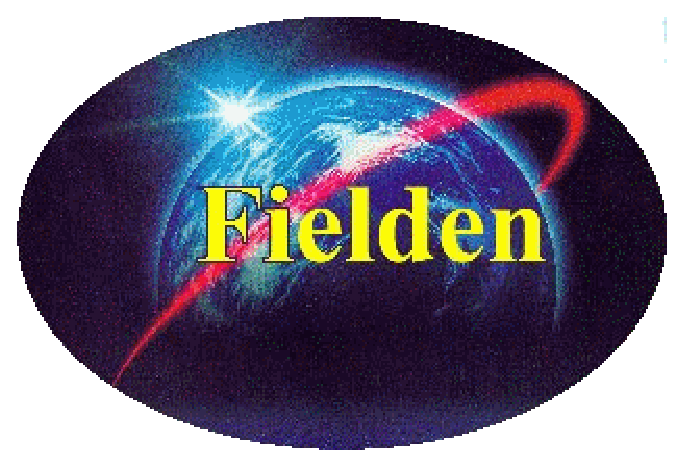
\includegraphics[scale=0.2]{images/04-logo}}
    \hspace{15em}
    \subfigure{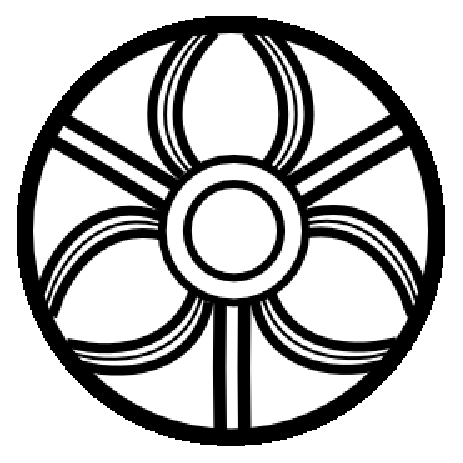
\includegraphics[scale=0.2]{images/03-logo}}
  \end{figure}
 \titlepage
  

}
%%%%%%%%%%%%%%%%%%%%%%%%%%%%%%%%%%%%%%%%%%%%%%%%%%%%%%%%%%%%%%%%%%%%%%%%%%%%%%%%%%
\section{Agenda}
\frame{
      \frametitle{Presentation Agenda}
      \large{
	\begin{itemize}
  	\item Existing issues with Client/Server application development methodology (Delphi)
  	\item Existing issues with web browser-based programming model (Java)
	\item Software vs. Domain Architecture
  	\item Domain-driven design (DDD)
	\item Trident Genesis (TG) -- the enterprise applications development platform
	\item TG vs. Others
	\item Development and deployment of new applications
	\item Technical details:  Code and UI
	\end{itemize}
      }
}

\section{Making of Software}

\frame{
      \frametitle{Existing issues with Client/Server application development methodology (Delphi)}
      \large{
	\begin{itemize}
  	\item High level of development complexity -- too much of tech details
	\item UI centric development (as most RAD tools)	
	\item Difficult to modify UI layout due to pixel precision positioning
        \item Data-driven application design (data-aware controls, data dependent business logic)
  	\item Does not encourage good development practices (patterns, unit testing, code reuse, refactoring)
	\item Often RDBMS dependency (SP + proprietary features)
	\end{itemize}
      }
}

\frame{
      \frametitle{Existing issues with web browser-based programming model (Java)}
      \large{
	\begin{itemize}
  	\item Browser dependency (e.g. different behaviours in IE and Firefox)  	
  	\item Complex development model (HTML, CSS, JavaScript, AJAX, web-framework...)
	\item Lack of UI richness and interactivity (HTML limitation)	
	\item Difficulties with horizontal scalability (session management)
	\item Still too much of technical details
	\end{itemize}
      }
}

\frame{
      \frametitle{Software vs. Domain Architecture}
      
      \large{
	\begin{spacing}{2.5}
	\begin{itemize}
	  \item Software architecture can be reused
	  \item Domain architecture is very often unique (customer specific)
	  \item Modeling of the business domain is the core value for customers
	\end{itemize}
	\end{spacing}
      }
}

\frame{
	\frametitle{Domain-Driven Design}	
	\noindent\Large{Software design approach based on two premises:}
	\large{
	\begin{itemize}
	\begin{spacing}{1.5}
  	\item Complex domain designs should be based on a business model	
  	\item The primary focus should be on the domain and domain logic, but not on a particular technology/architecture used to implement the application
	\end{spacing}
	\end{itemize}
	}
	
}

\section{Trident Genesis (TG) -- the enterprise applications development platform}
\frame{
	\frametitle{What is TG?}
	\noindent\Large{Trident Genesis is an enterprise applications development platform:}
	\large{
	\begin{itemize}
	\begin{spacing}{1.5}
  	\item Based on Domain-Driven Design paradigm
        \item Provides high level abstractions to hide software architecture complexity from application developers\\
              (bottom-up approach -- from domain definition to UI design)
	\item Scalable -- caters for development of small and large business applications
	\end{spacing}
	\end{itemize}
	}
}
\frame{
	\frametitle{Core Features I}
	\large{
	\begin{itemize}
  	\item Domain centric application development with a life cycle revolving around business entities and logic  	
	\item Fully resource oriented architecture (ROA)
        \item Good performance scalability (both horizontally and vertically)
	\item TG-based applications are automatically Rich Internet applications (RIA)
        \item Secure -- utilises Amazon S3 like approach to authentication  	
	\item Pluggable authorisation model (e.g. LDAP, DB-based), declaritive security
	\item High level degree of configuration
	
	\end{itemize}
      }
}
\frame{
	\frametitle{Core Features II}
	\large{
	\begin{itemize}
	\item Intensive utilisation of declarative and meta programming
        \item No code generation
	\item Ease of user interface (UI) development in a domain centric way
	\item Domain Query API (provides object-oriented means to query persisted domain entities) with built-in visual composer (Snappy)
	\item RDBMS independent
        \item Data auditing and role-based data visibility control
        \item Support for separation of development roles (domain logic and UI can be developed concurrently)
	\end{itemize}
      }
}
\frame{
	\frametitle{Main Advantages}
	\large{
	\begin{itemize}
	\item Pure Java, which reduces the learning curve (no need to know HTML, CSS, JavaScript and other browser-related technologies)
        \item Entry level development skills requirement 
	\item Improves application maintainability: code is limited mostly to domain definition and business logic
	\item Increases speed of development
	\item Applications are RIA/ROA
	\item Covers a complete development life cycle -- from DB to UI.
	\item OS and RDBMS independent
	\item Ensures data integrity automatically (handles concurrent modifications properly)
	\item Ready to be extended by 3rd party developers if required
	\end{itemize}
      }
}

\frame{
	\frametitle{Other solutions}
	\large{
	\begin{itemize}
	\begin{spacing}{1.5}
	\item Proprietary solutions: SAP, Maximo SAM, JD Edwards World, Microsoft Dynamics, 1C:Enterprise
	\item Open source solutions: OpenERP, Compiere, OFBiz, Openbravo
	\item The main characteristics:
	    \begin{itemize}
	       \item Data centric (tables and fields)
	       \item Proprietary 4GL-like limited (not general purpose) languages (e.g. SAP ABAP, Microsoft Axapta X++)
               \item Wizards for application configuration/generation
	    \end{itemize}
	\end{spacing}
	\end{itemize}
      }
}

\frame{
	\frametitle{TG vs. others solutions}
	\large{
	\begin{itemize}
	\begin{spacing}{1.5}
        \item Domain centric, based on object-oriented approach
	\item Pure Java (well known general purpose language) -- this ensures TG extensibility by 3rd parties (no vendor lock-in)
        \item No code generation -- easier maintenance
	\item Application is user configurable (layout, data view, analysis)
        \item Domain definition and logic are implemented by developers (skill set fusion)
	\end{spacing}
	\end{itemize}
      }
}

\frame{
	\frametitle{TG Principles}
	\large{
	\begin{itemize}
	\begin{spacing}{1.5}
	\item ``\ldots as simple as possible, but not simpler'' \emph{(Albert Einstein)}
        \item Prototyping/development agility (order of magnitude faster comparing to conventional Delphi/Java development)
	\item Maintainability
        \item Easy enhancement -- modifications
	\item Usability and UI consistency
	\end{spacing}
	\end{itemize}
      }
}


\frame{
  \frametitle{Deployment of TG-based applications}
  \begin{figure}
    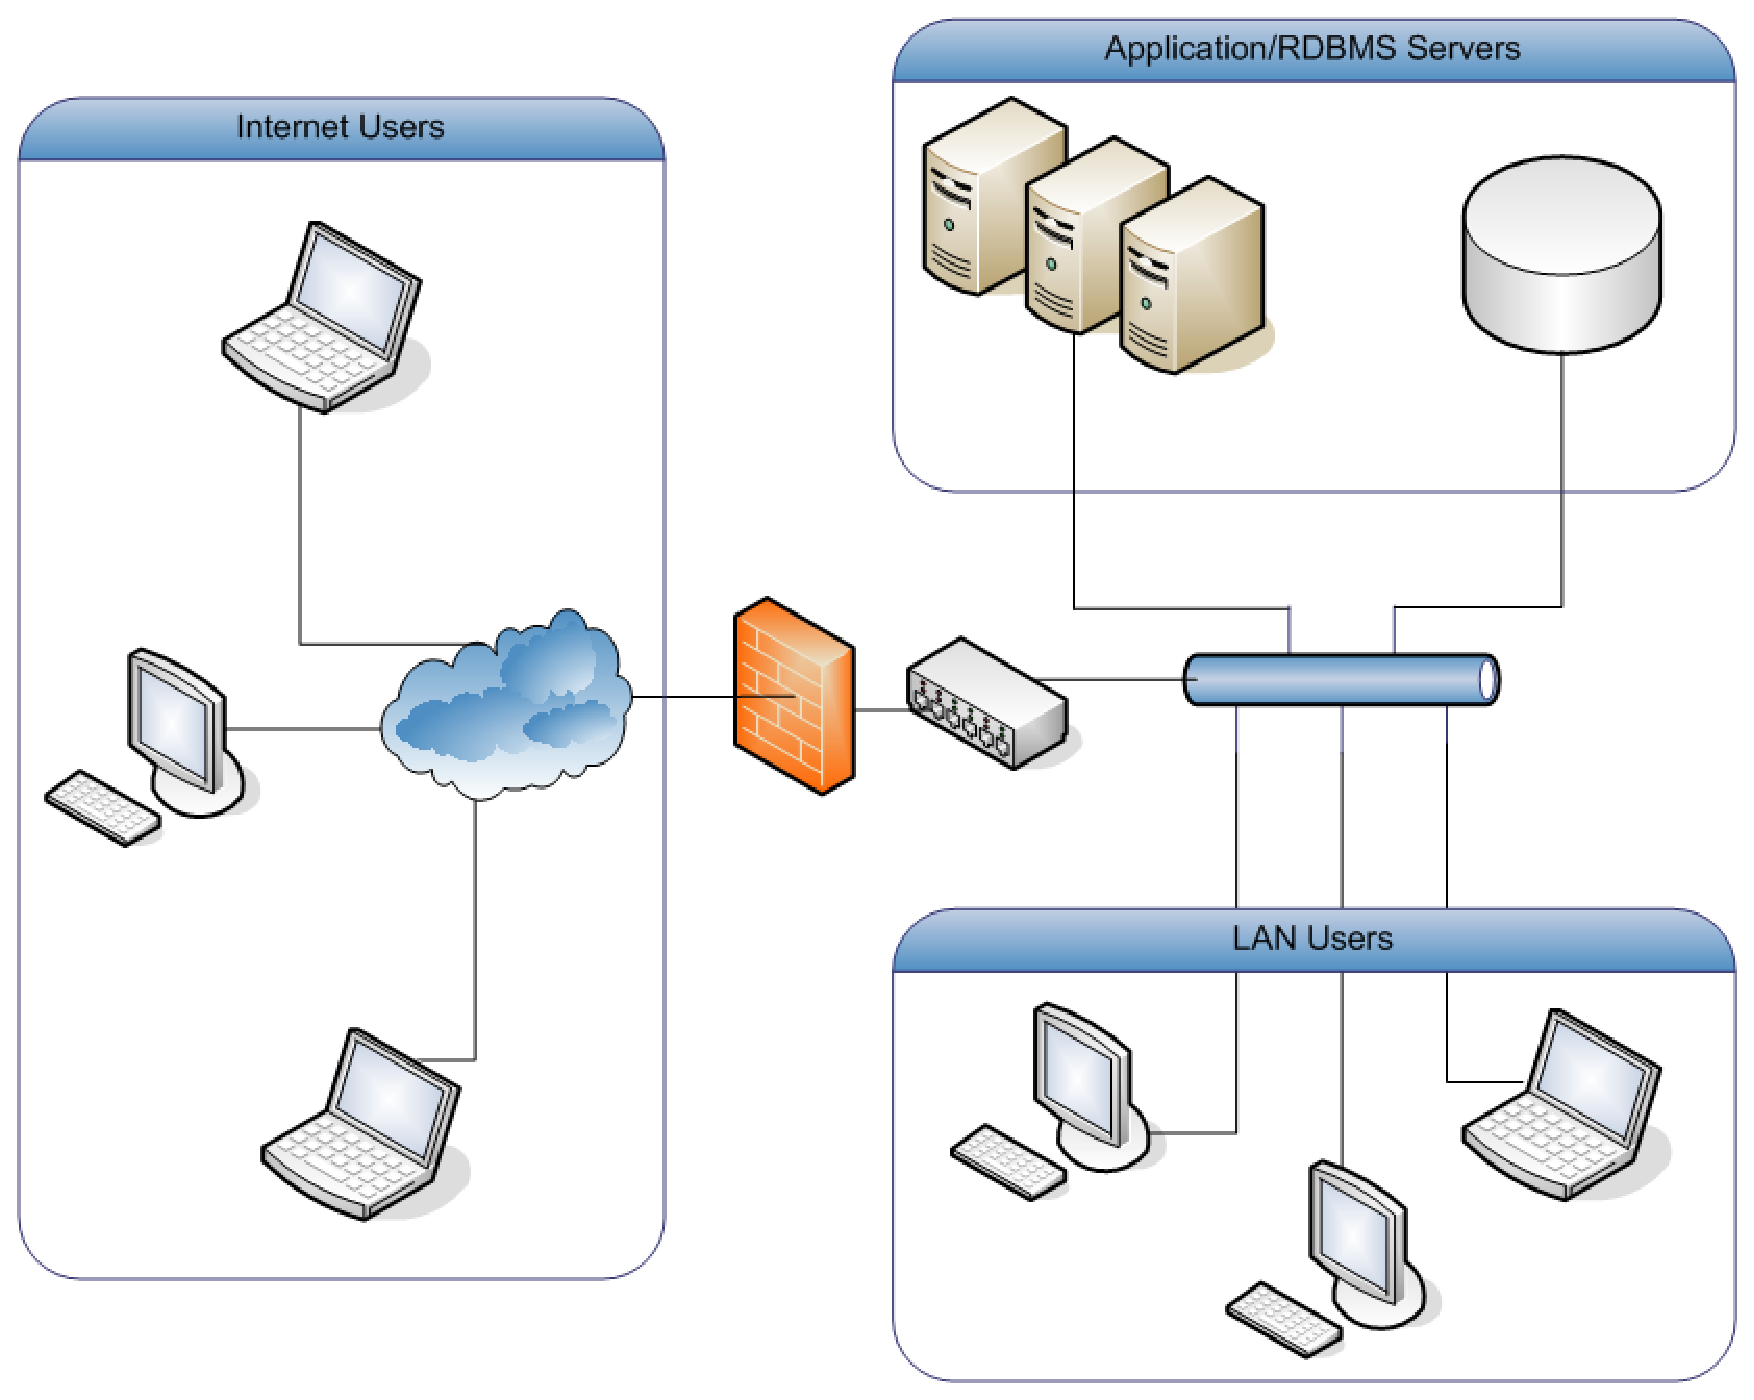
\includegraphics[scale=0.31]{images/01-tg-based-app-deployment}
  \end{figure}
}

\frame{
  \frametitle{Typical modules of TG-based applications\\(weak coupling)}
  \begin{figure}
    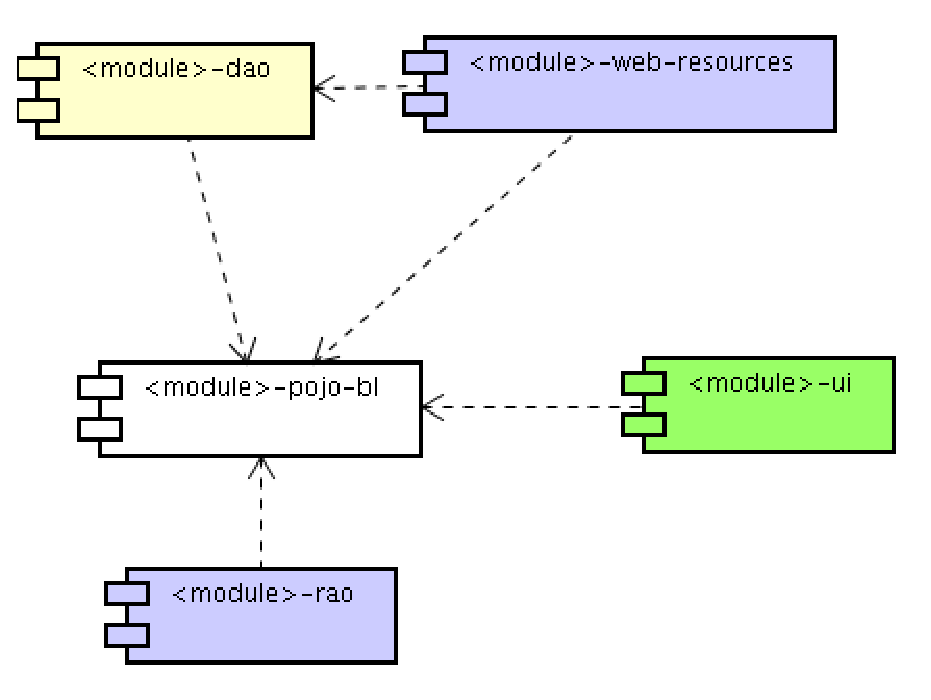
\includegraphics[scale=0.5]{images/02-inner-module-dependencies}
  \end{figure}
}


\begin{frame}[fragile]
  \frametitle{Technical details: Code and UI}  
  \noindent\Large{Show screencasts:}
  \large{
	\begin{itemize}
	\begin{spacing}{1.5}
	\item Property title modification (01-tg-based-app-title-change-demo.avi)
        \item Domain enhancement (02-tg-based-app-domain-enhancement.avi)
	\item UI enhancement (03-tg-based-app-domain-enhancement-master.avi)
	\end{spacing}
	\end{itemize}
  }
\end{frame}

\begin{frame}[fragile]
  \frametitle{Domain Query API vs. SQL}   
  %Is a library
  \noindent\Large{Domain Query API:}
  \begin{lstlisting}
      IQueryOrderedModel qm = new select(WorkOrder.class).where().the("vehicle.station.key").in("A09","A10","A11")
                              .and().the("customer.key").eq("NSWA").ordeBy("transDate desc").model();
      List<WorkOrder> workOrders = woDao.getPage(qm, 0, 25).data();
  \end{lstlisting}
  \noindent\Large{SQL:}
  \begin{lstlisting}[language=SQL]
    SELECT
        _WorkOrder_0.*        
    FROM
        WODET _WorkOrder_0 
    LEFT JOIN
        EQDET _vehicle_0_1 ON _vehicle_0_1._ID = _WorkOrder_0.ID_EQDET 
    LEFT JOIN
        ORG_LEVEL4 _station_0_2 ON _station_0_2._ID = _vehicle_0_1.ID_ORG_LEVEL4 
    LEFT JOIN
        CUSTOMERS _customer_0_1 ON _customer_0_1._ID = _WorkOrder_0.ID_CUSTOMERS    
    WHERE
        _customer_0_1.KEY_ = 'NSWA' AND _station_0_2.KEY_ IN ('A09', 'A10', 'A11')
    ORDER BY
        _WorkOrder_0.TRANS_DATE DESC limit 25
  \end{lstlisting}
\end{frame}

  


\end{document}